
\section{Neural Net Backprop Gradient Derivation (15 points)}

\begin{figure}[h]
\centering
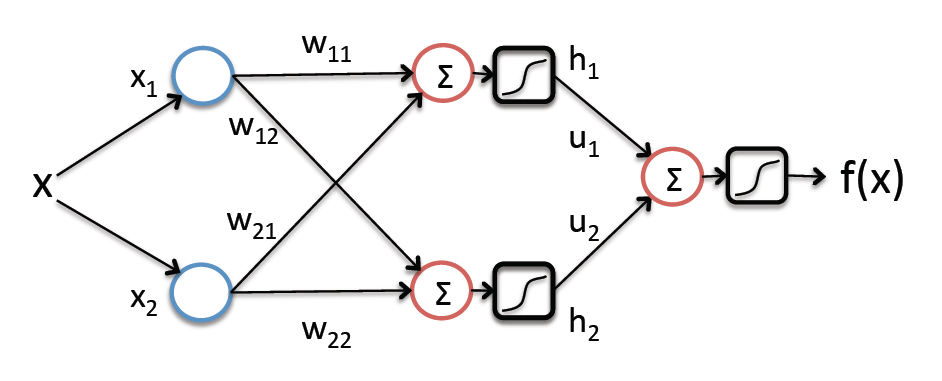
\includegraphics[scale=0.27]{image/neural_net_1.png}
\vspace{-0.1in}
\caption{Illustration of Simple Neural Network.}
\label{fig:neuralnet}
\end{figure}

In this question, we will consider the following neural network depicted in Figure \ref{fig:neuralnet}.  There are six parameters in the model, $u_1$, $u_2$, $w_{11}$, $w_{21}$, $w_{12}$, and $w_{22}$.

The network takes in a 2-dimensional input $x$ and outputs a real value $f(x) \in [0,1]$.  The final output $f(x)$ is a weighted combination of two hidden node activations with a sigmoid transfer function:
\begin{eqnarray}
f(x) = \sigma \left(\sum_{i=1}^2 u_i h_i(x) \right),
\end{eqnarray}
where:
$$\sigma(s) = \frac{e^s}{1+e^s},\ \ \ \ \ \ \ \ \ \ \ \mbox{and}\ \ \ \ \ \ \ \ \ \ \ \ 
h_i(x) = \sigma\left(\sum_{j=1}^2 w_{ji} x_j\right).$$

\smallskip

\textbf{Question 1:} (5 points)
For a given training data point $(x,y)$, compute the stochastic gradient of the squared-loss of $(x,y)$ w.r.t. $w_{11}$:
$$\frac{\partial}{\partial w_{11}} L(y,f(x)) \equiv \frac{\partial}{\partial w_{11}}\left(y - f(x)\right)^2.$$

Hint: write the formula using the chain rule and use the following definition of the derivative of $\sigma(s)$:
$$\frac{\partial}{\partial s}  \sigma(s) = \sigma(s)(1-\sigma(s)).$$
\bigskip

\textbf{Question 2:} (5 points)
Find $\frac{\partial}{\partial w_{11}} L(y,f(x))$ where:
$$(x, y) = ((0.1, 0.5), 0.75)$$
$$(u_1, u_2) = (0.5, -0.1)$$
$$(w_{11}, w_{12}, w_{21}, w_{22}) = (0.25, 0.1, 0.05, -0.25)$$
\smallskip

\textbf{Question 3:}  (5 points)
Use your derivations from the previous two questions to identify which term in the gradient derivation results in the vanishing gradient problem, and briefly explain how the problem is exacerbated in neural networks with more layers.
\smallskip


